

\documentclass{beamer}

% Relating Momentum "Impulse" to input velocities for landing envelope constraints. 

% \usepackage{beamerthemesplit} // Activate for custom appearance

%\renewcommand{\vec}[1]{\mathbf{#1}}

%\newcommand{\vectormit}[3]{{^{\mathcal{#2}}\vec{#1}^{#3}}} 

%\title{Power Loss Equations}
%\author{Estrada}
%\date{\today}
\usepackage{eurosym}
\usepackage{enumerate}
\usepackage{multirow}
\usepackage{amsmath}
\begin{document}



%\frame{\titlepage}

%\section[Outline]{}
%\frame{\tableofcontents}

%\section{Introduction}
%\subsection{Overview of the Beamer Class}


\title{Tuning Wrist Compliance for Curved Surface Gripper with Adhesion Limitations}
\subtitle{}
\author{Matt\newline FBD from and discussions w/ Elliot}

\frame
{
\titlepage
 }

\frame
{
\frametitle{FBD}

FBD from Elliot/Hao model shows four vectors. Tension from the adhesive film is oriented tangent to the surface, and compressive forces are oriented normal to the surface. 

Point $N_{0}$ is located at the center of the gripper's structure. 
Point $B_{cm}$ is located at the body's center of mass. 

\begin{figure}[htb]
	\centering
	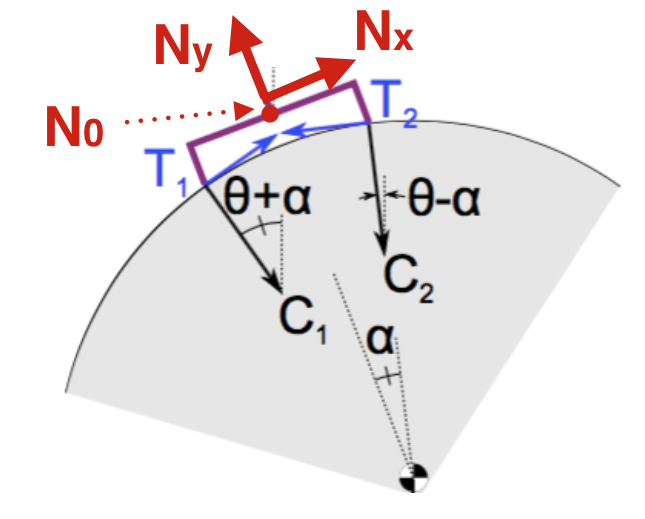
\includegraphics[width=2.25in]{images/gripperLabel.png}
	\caption{Defining axes off Elliot's FBD.}
	\label{fig:FBD}
\end{figure}
}


\frame
{
\frametitle{Force Vectors}

Vectors directions as a function of $\alpha$, for the 2D case.  

%\begin{align*}
%t_{1} = [\cos{\alpha} , \sin{\alpha}, -r ]^{T}	\\
%t_{2} = [-\cos{\alpha} , \sin{\alpha}, r ]^{T}	\\
%c_{1} = [\sin{ \alpha } , -\cos{ \alpha }, 0 ]^{T}	\\
%c_{2} = [-\sin{ \alpha } , -\cos{ \alpha }, 0 ]^{T}	\\ 
%\end{align*}

Where unit vectors are defined as: 

\begin{equation}
\hat{t_{1}} =
\begin{bmatrix}
           \cos{\alpha}  \\
           \sin{\alpha} \\
           -r \\
\end{bmatrix} =
 \frac{1}{||T_{1}||}
\begin{bmatrix}
           \vec{T_{1}} \cdot \hat{n_{x}}  \\
           \vec{T_{1}} \cdot \hat{n_{y}} \\
           \vec{-r}\,  x \vec{T_{1}} \cdot \hat{n_{z}} \\
\end{bmatrix} 
\end{equation}
         
Where compressive forces are denoted $c_{1}$, $c_{2}$, and tension in adhesive is denoted  $t_{1}$, $t_{2}$.

Putting this in a matrix format yields: 

\begin{equation}
A =  [\hat{t_{1}} \,\,  \hat{t_{2}}\,\,  \hat{c_{1}}\,\,   \hat{c_{2}}]
\end{equation}
	
Where A is ${\rm I\!R} ^{m x n}$ in this 2D case. We have $m$ = 3 DOF and $n$ = 4 force vectors.
}


\frame
{
\frametitle{ Net Force }


Net force of body B is a function of A, since 

\begin{equation}
	F_{net} = A * x
\end{equation}


Where $F_{net} = [F_{x}, F_{y},  M_{z}]^{T}$ is the net forces and moment on the object along the directions $[n_{x}, n_{y}, n_{z}]$.  $M_z$ is the net moment on rigid body B, taken about $B_{cm}$.

Vector x, (sized ${\rm I\!R} ^{n x 1}$), represents magnitude of each of the forces. We essentially get to turn $n$ knobs in our simulation, (each entry of x). 

\begin{equation}
	a_{net} = m^{-1}A * x
\end{equation}

Net force is proportional to net acceleration, just scaling by mass/Inertia in each line m = diag(mB, mB, Icm). 
	
}


\frame
{
\frametitle{ Convex Optimization Problem }

If we assume $ F_{net} = \beta*d $ we can choose a general proportion of net forces d, ${\rm I\!R} ^{3 x 1}$,  and maximize its magnitude, $\beta$ .
	
\begin{equation*}
	\begin{aligned}
	& \underset{x}{\text{maximize}}
	& & \beta \\
	& \text{subject to}
	& & F_{net} = A * x \\
	&
	& & 0 \leq x \leq x_{max}
	\end{aligned}
\end{equation*}

Our adhesion limitations, and any structural limitation we would put on the compressive forces are contained in $x_{max}$. To clarify:  

\begin{equation*}
x = 
\begin{bmatrix}
           \,\, ||\vec{T_{1}}|| \,\,\\
           ||\vec{T_{2}}|| \\
           ||\vec{C_{1}}|| \\
           ||\vec{C_{2}}|| \\
\end{bmatrix} 
x_{max} = 
\begin{bmatrix}
           adhesive1_{max} \\
           adhesive2_{max} \\
           contact1_{max} \\
           contact2_{max} \\ 
\end{bmatrix} 
F_{net} = 
\begin{bmatrix}
           \Sigma F_{x} \\
           \Sigma F_{y}\\
           \Sigma M_{z}\\
\end{bmatrix} 
\end{equation*}	
}


\frame
{
\frametitle{ Convex Optimization Problem }

	
\begin{equation*}
	\begin{aligned}
	& \underset{x}{\text{maximize}}
	& & \beta \\
	& \text{subject to}
	& & F_{net} = A * x \\
	&
	& & 0 \leq x \leq x_{max}
	\end{aligned}
\end{equation*}

For instance, imposing $d = [1, 0, 0]^{T}$ would be to accelerate the object in a purely horizontal direction without rotating the object at all. 

$d = [0, 0, 1]^{T}$ would be to rotate the object without moving it's COM. 
	
}


\frame
{
\frametitle{ Sweep of Adhesion Capabilities }

We can find the maximum acceleration that we can exert on the object in different directions by sweeping this maximization problem. 

\begin{figure}[htb]
	\centering
	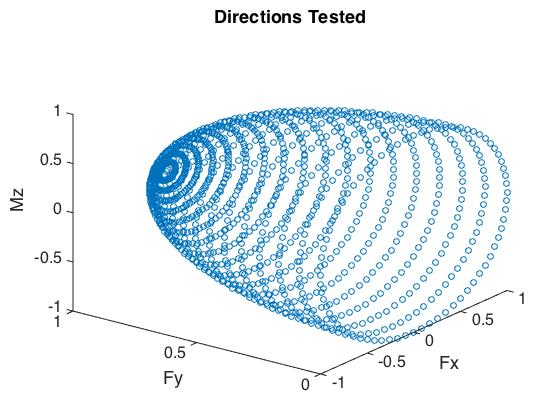
\includegraphics[width=2.25in]{images/directions.jpg}
	\caption{This is just a plot of a unit dome, showing the directions I'm "tugging" the object.}
	\label{fig:directions}
\end{figure}
	
}


\frame
{
\frametitle{ Adhesion Capabilities }

We can find the maximum forces (probably easier to think of this as max achievable accelerations) that we can exert on the object in different directions by sweeping this maximization problem. 

\begin{figure}[htb]
	\centering
	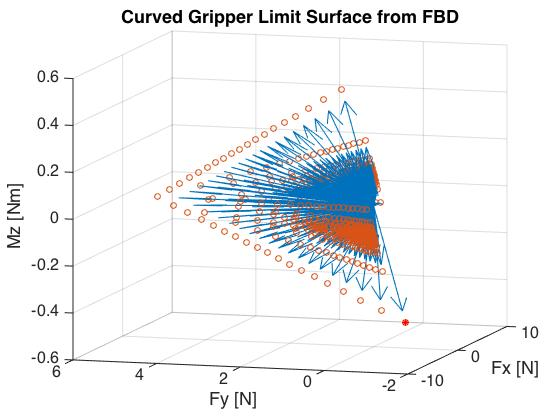
\includegraphics[width=2.25in]{images/CurvedGripperFBDSurfaceLimit.jpg}
	\caption{Point cloud of maximum net forces/moment able to be exerted on object in different directions. Anything contained within the boundary is fair game.}
\end{figure}
	
}


\frame
{
\frametitle{ Horizontal and Rotational Accelerations  }

More manageable to think about is a 2D slice, for instance, what horizontal accelerations you can exert with different rotations. 

\begin{figure}[htb]
	\centering
	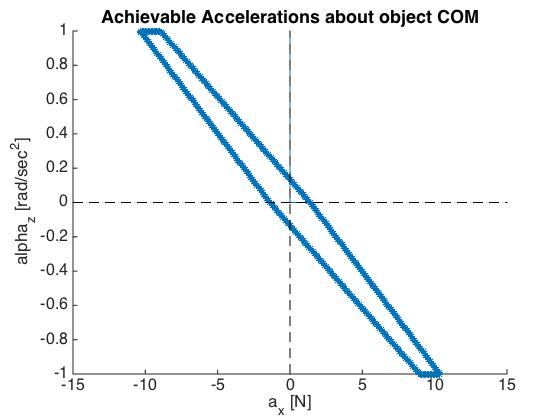
\includegraphics[width=2.25in]{images/AxAzAccelerations.jpg}
	\caption{Point cloud of maximum accelerations able to be exerted on object in different directions.}
	\label{fig:accel}
\end{figure}

Everything within this loop is attainable by the specified adhesion/geometry. 
	
}


\frame
{
\frametitle{ Varying $\alpha$}

What happens if we vary how far around the object we are contacting? $\alpha$ is denoted in degrees: 

\begin{figure}[htb]
	\centering
	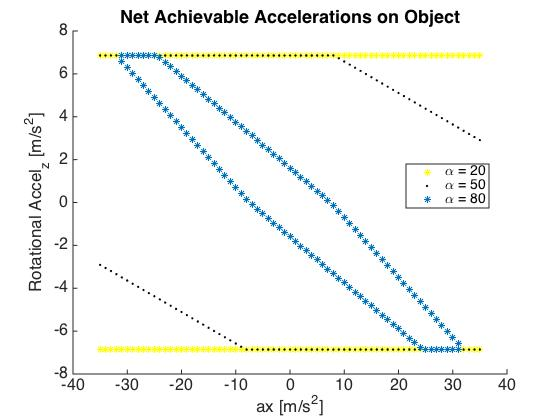
\includegraphics[width=2.25in]{images/VaryingAlpha.jpg}
	\caption{Same constraints on adhesion, just varying geometry, $\alpha$.}
\end{figure}
	These limits should be shaded regions. For instance, yellow ($\alpha$ = 80 degrees) is a rectangle in this space. 
}

\frame
{
\frametitle{ Varying $\alpha$ Interpretation}


\begin{figure}[htb]
	\centering
	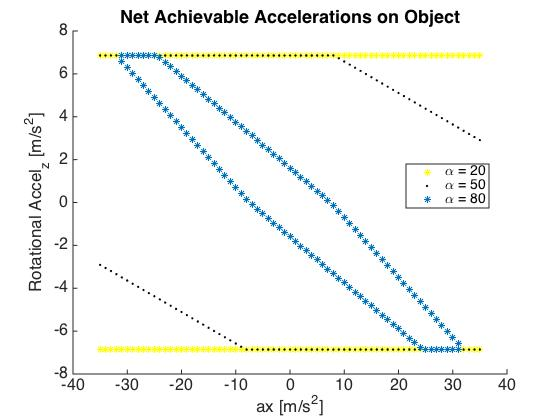
\includegraphics[width=2.25in]{images/VaryingAlpha.jpg}
	\caption{Same constraints on adhesion, just varying geometry, $\alpha$.}
\end{figure}
	
	As alpha converges to zero, the ability to move your object tangentially and rotating the object become more coupled. A single force vector acting at a radius would be a diagonal line in this graph. 
}


\frame
{
\frametitle{ Moment and Tangential Force  }

Assuming the gripper/object are a rigid body, we can back out what force would be required to achieve a given acceleration.

The forces/torque applied at a given point p, to impose an acceleration a, are given as

\begin{equation}
F_{p} = 
  -\begin{bmatrix}
    1 & 0 & 0 \\
    0 & 1 & 0 \\
    (r+d) & 0 & 1 \\
  \end{bmatrix}
* a
\end{equation}

Variable r is the radius of the object, and d is the offset between the surface of the curved object and the wrist of the gripper at point $N_{0}$. 
	
}


\frame
{
\frametitle{ Sustainable Forces and Torques at a Given Point}

Taking the accelerations shown to be achievable in Fig. \ref{fig:accel}, we see the forces and moment applied at the wrist that are within the adhesive's capability. 

\begin{figure}[htb]
	\centering
	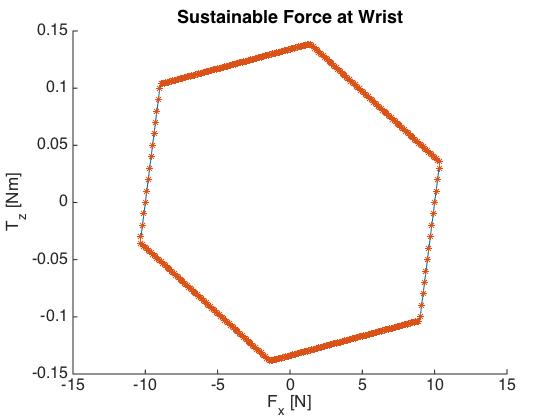
\includegraphics[width=2.25in]{images/FxMzForces.jpg}
	\caption{Point cloud of maximum forces/moments able to be exerted on object in different directions.}
\end{figure}
	
}


\frame
{
\frametitle{ Wrist Design }

Unless we make passive wrist compliance a function of orientation, there is no guarantee that Fx will not attain its max value at the same time Tz attains its max value. 
So say Fx could be anywhere between $\pm$ 10 and $T_{z}$ might be anywhere between $\pm$ 0.5.

\begin{figure}[htb]
	\centering
	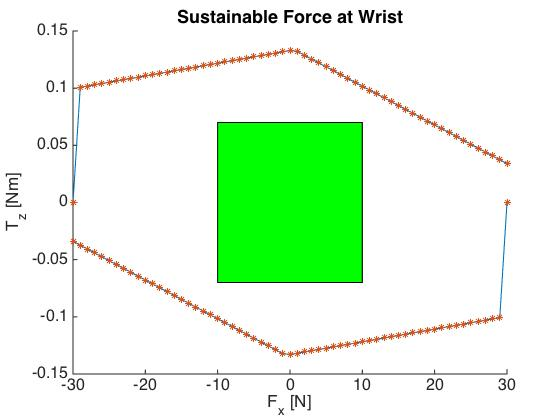
\includegraphics[width=2.25in]{images/WristCompliance2D.jpg}
	\caption{}
\end{figure}

}

\frame
{
\frametitle{ Wrist Design Interpretation }

Possibility of forces transmitted by a compliant wrist capable of transmitting those forces would be the space enclosed by the square here. 

\begin{figure}[htb]
	\centering
	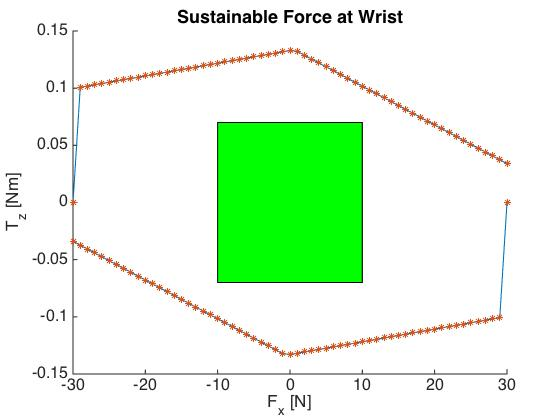
\includegraphics[width=2.25in]{images/WristCompliance2D.jpg}
	\caption{}
\end{figure}

Note we would miss out on a sizable area in our achievable force/moment space. Active control could attain this. Appreciable inertia's/damping would vary from this in impacts. 

}


\frame
{
\frametitle{ Wrist Design Envelope}

Bringing this to consider all three variables again, that patch of possible forces exerted by the wrist will turn into a cube. 

\begin{figure}[htb]
	\centering
	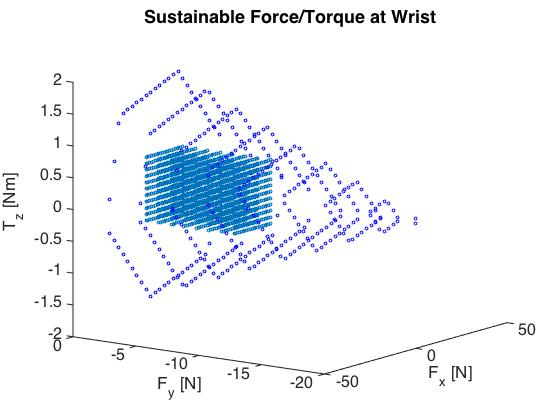
\includegraphics[width=2.25in]{images/WristConstraints.jpg}
	\caption{}
\end{figure}

If the cube extends beyond this funnel, adhesion capabilities will be exceeded. 

}

\frame
{
\frametitle{Optimize Losing Kinetic Energy}

\begin{equation*}
	\begin{aligned}
	& \underset{x}{\text{maximize}}
	& & P = \vec{F_{net} } \cdot \vec{v} \\
	& \text{subject to}
	& & F_{net} = A * x \\
	&
	& & 0 \leq x \leq x_{max}
	\end{aligned}
\end{equation*}

}

\frame
{
\frametitle{ Questions/FutureWork }

\begin{itemize}

	\item Write out A and A*Translation symbolically
	\item Does Pivot Joint Really Count as pure Torque? Not if robot COM is cantilevered off the axis of rot. 
	\item SVD, Eigenvalues, Nullspace
	\item What are these corners in graphs coming from? 
	\item Explore potential adhesive layout cases, like lobster claw asymmetry where one side is stronger. 
	\item Expand to 3D gripper for Hao, curved vs flat grip? 
\end{itemize}

}

\frame
{
\frametitle{ Questions/FutureWork }

\begin{itemize}


	\item Quantify "safety margin"? Cost function, or prioritizing one measure? 
	\item Any way to maximize layout based on an optimization? Can I get a measure of space enclosed in convex hull? 
	\item Can we take a bunch of data and do a least squares fit? I guess we'd only be optimizing for allowable value of T
	\item Can we use A as a ''jacobian" to direct us to a more sustainable posture? Double check which vectors in x are closest to limitations. 
	\item Shade limitations based on which adhesive was going to fail. 
	\item Gripper Design for Specific Target Objects (would this want to be alpha=45 if we knew radius?)	
	
\end{itemize}

}


\end{document}
